%
%\documentclass[fleqn]{report}
%\usepackage{graphicx} % om PostScript plaatje in te lassen
%\usepackage{here}     % voor geforceerde plaatsing figuren
%\usepackage{amsmath}
%\textwidth=17.0cm
%\textheight=22.0cm
%\topmargin=-1cm
%\oddsidemargin=-0.3cm
%\evensidemargin=-0.3cm
%
%%packages
%\usepackage{amsmath}
%\usepackage{cite}
%\usepackage[toc,page]{appendix}
%\usepackage{fancyvrb}
%\usepackage{tikz}
%\usepackage{multicol}
%\usepackage{framed}
%\usepackage{pgfplots}
%\usepackage{fixltx2e}
%\usepackage{subfigure}
%\usepackage{lscape}
%\usepackage{enumitem}
%\usepackage{filecontents}
%\usepackage{multicol}
%
%
%%tikz labraries
%\usetikzlibrary{matrix}
%\usetikzlibrary{decorations.pathreplacing}
%\usetikzlibrary{positioning}
%\usetikzlibrary{calc}
%\usetikzlibrary{shapes,arrows, chains}
%\usetikzlibrary{intersections}
%\usetikzlibrary{decorations.markings}
%\usetikzlibrary{calc,intersections}
%%\usetikzlibrary{decorations.pathreplacing,bending}
%
%% define mathcolor
%\makeatletter
%\def\mathcolor#1#{\@mathcolor{#1}}
%\def\@mathcolor#1#2#3{%
%  \protect\leavevmode
%  \begingroup
%    \color#1{#2}#3%
%  \endgroup
%}
%\makeatother
%
%%extra instellingen
%\newlist{aims}{enumerate}{1}
%\setlist[aims,1]{
%  label={*},
%  leftmargin=*,
%  align=left,
%  labelsep=2mm,
%}
%
%\newlist{aims2}{enumerate}{1}
%\setlist[aims2,1]{
%  label={},
%  leftmargin=0pt,
%  align=left,
%  labelsep=4mm,
%}
%
%\newlist{aims3}{enumerate}{1}
%\setlist[aims3,1]{
%  label={-},
%  leftmargin=2cm,
%  align=left,
%  labelsep=0.4mm,
%}
%
%\usepackage{pgfplots}
%
%\begin{document}

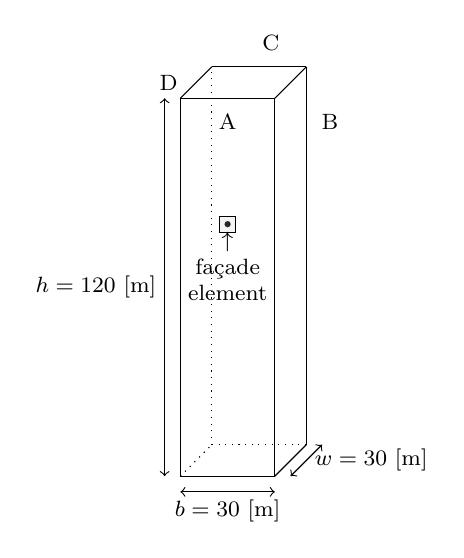
\begin{tikzpicture}[scale=10]
\footnotesize
\draw (-0.06,0) rectangle (0.06,0.480);
\draw (0.06,0) -- (0.10,0.04);
\draw (0.06,0.480) -- (0.10,0.52);
\draw (-0.06,0.480) -- (-0.02,0.52);
\draw (0.10,0.04) -- (0.10,0.52);
\draw (-0.02,0.52) -- (0.10,0.52);
\draw [dotted] (-0.06,0) -- (-0.02,0.04);
\draw [dotted] (-0.02,0.04) -- (0.1,0.04);
\draw [dotted] (-0.02,0.04) -- (-0.02,0.52);

% height
\draw [<->] (-0.08,0) -- (-0.08,0.480) node [midway, anchor=east] {$h = 120$ [m]};
% width
\draw [<->] (-0.06,-0.02) -- (0.06,-0.02) node [midway, anchor = north] {$b = 30$ [m]};
% depth
\draw [<->] (0.08,0) -- (0.12,0.04) node [midway, anchor = west] {$w = 30$ [m]};

%\draw [->] (-0.1,0) -- (-0.1,0.12);
%\node [left ] at  (-0.07,0.12) {$z$};
% x-distance
%\draw [<->] (-0.06,0.37) -- (0,0.37) node [midway, anchor = south] {x = 24 [m]};
% z-distance
%\draw [<->] (-0.03,0) -- (-0.03,0.32) node [midway, anchor = west] {$z = 80$ [m]};

\node at (0,0.45) {A};
\node at (0.13,0.45) {B};
\node at (0.055,0.55) {C};
\node at (-0.075,0.5) {D};
\draw (0,0.320) node[circle,fill,inner sep=0.8pt,align=center, label=below:]  (1) {};
\node [below, align=center] at (0,0.32) {$\uparrow$ \\ fa\c{c}ade \\ element};

\draw [fill=black!20, fill opacity=0.2] (-0.01,0.31) rectangle (0.01,0.33);


%\draw (-0.06,0.320) -- (0.06,0.32);
%\draw (0.06,0.320) --  (0.10,0.36); 


\end{tikzpicture}
%
%\end{document}